\documentclass[a4paper,15pt]{jsarticle}

% 数式
\usepackage{amsmath,amsfonts}
\usepackage{bm}
% 画像
\usepackage[dvipdfmx]{graphicx}

\usepackage{here}
\usepackage{url}

\usepackage{listingsutf8,jlisting} %日本語のコメントアウトをする場合jlistingが必要
%ここからソースコードの表示に関する設定
\lstset{
  basicstyle={\ttfamily},
  identifierstyle={\small},
  commentstyle={\smallitshape},
  keywordstyle={\small\bfseries},
  ndkeywordstyle={\small},
  stringstyle={\small\ttfamily},
  frame={tb},
  breaklines=true,
  columns=[l]{fullflexible},
  numbers=left,
  xrightmargin=0zw,
  xleftmargin=3zw,
  numberstyle={\scriptsize},
  stepnumber=1,
  numbersep=1zw,
  lineskip=-0.5ex
}

\begin{document}

\title{コンピュータ科学実験レポート}
\author{坪井正太郎(101830245)}
\date{\today}
\maketitle

\section*{はじめに}

\section*{各実験}
% \section{実験1-1}
\subsection{実験の目的、概要}
この実験では、ディスプレイに'B'を表示させるMIPSマシンコードを、MIPSプロセッサを再現したFPGA上で実行する。
その際、事前にプロセッサの動作について予想しておき、結果と比較する。

これによって、メモリイメージファイルの生成方法、メモリイメージファイルから機械語を読んで実行結果を予測する方法を確認することを目的とする。

\subsection{実験方法}
\subsubsection{メモリイメージファイルの作成}
中身が以下のようなバイナリファイルprint\_B.binを配置した。
\lstinputlisting[caption=print\_B.bin,label=printB.bin]{src/01/print_B}

以下のコマンドでROM配置用のイメージファイルと、機能レベルシュミレーション用のverilog HDL記述ファイルを生成した。
\begin{lstlisting}[caption={イメージファイルの作成},label={イメージファイルの作成1-1}]
  $ bin2v print_B.bin
\end{lstlisting}

\subsubsection{命令列の確認}
生成されたrom8x1024\_sim.vを参照し、以下の点について結果を予測した。
\begin{itemize}
  \item PC=0x002cの命令を実行したときの、REG[2]の値
  \item PC=0x0030の命令を実行したときの、RAMの768番地の値
  \item PC=0x0034の命令を実行したときの、REG[3]の値
  \item PC=0x003cの命令を実行したとき、RAMの何番地の値がどう変化するか
  \item PC=0x0048の命令を実行したとき、RAMの何番地の値がどう変化するか
\end{itemize}

\subsubsection{論理合成}
以下を実行し、mips\_de10-lite.tar.gzを解凍し、その中にメモリのイメージファイルを配置してコンパイルした。

ACケーブル、モニタへのVGAケーブル、PCへのUSB接続、の順に行なったのち、モニタ電源をオンにした。
以下のコマンドで、PCでの接続状況を確認し、FPGAにダウンロードした。
\begin{lstlisting}[caption={論理合成操作},label={論理合成操作1-1}]
  $ tar -xvfz ./mips_de10-lite.tar.gz
  $ mv ./rom8x1024.mif ./mips_de10-lite/
  $ cd mips_de10-lite/
  $ quartus_sh --flow compile MIPS_Default
  $ dmesg
  $ quartus_pgm MIPS_Default.cdf
\end{lstlisting}

スイッチ0、1をonにして手動モードに切り替えた。
KEY0を押し、プロセッサをリセットした。
KEY1でカウンタを進めて、予想した点について動作を確認した。

\subsection{実験結果}
\subsubsection{メモリイメージファイルの作成}
\ref{printB.bin}の操作によって、rom8x1024\_sim.vと、rom8x1024.mifが生成された。
内容は以下のように、ROMへのアクセスと応答をエミュレーションしたシュミレーションファイルと、実際に命令列を配置するためのイメージファイルだった。

\lstinputlisting[caption=rom8x1024\_sim.v,label=rom8x1024sim.v1-1]{./src/01/rom8x1024_sim.v}
\lstinputlisting[caption=rom8x1024.mif,label=rom8x1024.mif1-1]{./src/01/mips_de10-lite/rom8x1024.mif}


\subsubsection{命令列の確認}
生成されたrom8x1024\_sim.v(ソースコード\ref{rom8x1024.mif1-1})を参照し、以下のように予想した。

\begin{itemize}
  \item PC=0x002cの命令を実行したときの、REG[2]の値
  \begin{itemize}
    \item ゼロレジスタと768の加算が代入されるので、768(=0x00000300)
  \end{itemize}
  \item PC=0x0030の命令を実行したときの、RAMの768番地の値
  \begin{itemize}
    \item ゼロレジスタの値が代入されるので、0
  \end{itemize}
  \item PC=0x0034の命令を実行したときの、REG[3]の値
  \begin{itemize}
    \item 772が代入されるので、772
  \end{itemize}
  \item PC=0x003cの命令を実行したとき、RAMの何番地の値がどう変化するか
  \begin{itemize}
    \item REG[3]→772で、REG[2]→2なので、RAM[772]が2になる
  \end{itemize}
  \item PC=0x0048の命令を実行したとき、RAMの何番地の値がどう変化するか
  \begin{itemize}
    \item PC=0x0030でRAM[REG[2]→768]=0なので、RAM[768]が0→1になる
  \end{itemize}
\end{itemize}

\subsubsection{論理合成、FPGAでの回路実現}
手動でクロックを進めたが、画面には何も表示されなかった。
addiu命令と、sw命令が実装されていないので、予想した点について正しく実行される命令はなかった。

\subsection{考察}
addiuと、sw命令が実装されておらず、予想した時点で対応する命令コードを解釈できないので、何も実行されなかった。

また、目的であるイメージファイルの生成と、アセンブリの動作について確認することができた。

% \section{実験1-2}
\subsection{実験の目的,概要}
この実験では,実験1-1で正しく動作しなかったプロセッサに,新たに命令実装を追加し,同じプログラムを実行,結果を確認する。
また,実験1-1で行った予想と比較する。

これによって,プロセッサに命令を追加する方法,配線図を実装に反映させる方法を確認する。

\subsection{実験方法}
\subsubsection{addiu命令の追加設計}
以下の点について,main\_ctrl.vを編集した。
\begin{lstlisting}[caption={addiu命令の追加設計},label={addiu命令の追加設計}]
// 命令コードの定義を追加
`define ADDIU 6'b001001

// 分岐判定のコントロール信号を追加
`ADDIU: is_branch_ctrl_tmp = 3'b110;

// オペランドに即値,レジスタのどちらをとるのかの制御信号の追加
`ADDIU: alu_b_sel1_s_tmp = 1'b1;

// 即値の符号拡張が行われるかどうかのフラグを追加
(op_code == `ADDIU)

// ALUがどの演算を行うかの制御信号の追加
`ADDIU: alu_op_tmp = 3'b000;

// レジスタへの書き込み制御信号を追加
`ADDIU:  reg_write_enable_tmp = 1'b1;

// ALUの演算結果とRAMの内容のセレクト信号を追加
`ADDIU:  alu_ram_sel_s_tmp = 1'b0;

// RtとRdのセレクト信号の追加
`ADDIU:  reg_widx_sel1_s_tmp = 1'b0;

// レジスタに書き込む,ALUの出力orRAMのデータと,PCの値のセレクタ信号の追加
`ADDIU:  link_tmp = 1'b0;

\end{lstlisting}

\subsubsection{sw命令の追加設計}
以下の点について,main\_ctrl.vを編集した。
\begin{lstlisting}[caption={sw命令の追加設計},label={sw命令の追加設計}]
// 命令コードの定義を追加
`define SW 6'b101011 // store word (I 形式)

// RAMへの書き込みを制御する信号を追加
assign ram_write_enable = (op_code == `SW) ? 1'b1 : 1'b0;

// 分岐判定のコントロール信号を追加
`SW: is_branch_ctrl_tmp = 3'b110; // do nothing

// 即値とRtレジスタのセレクト信号を追加
`SW: alu_b_sel1_s_tmp = 1'b1;

// 即値の符号拡張が行われるかどうかのフラグを追加
|| (op_code == `SW)

// ALUがどの演算を行うかの制御信号の追加
`SW: alu_op_tmp = 3'b000;

// レジスタへの書き込み制御信号の追加
`SW: reg_write_enable_tmp = 1'b0;

\end{lstlisting}

\subsubsection{論理合成,FPGAでの回路実現}
以下のように,コンパイルを行ない,dmesgで接続を確認した。
その後FPGAにダウンロードして,FPGAでの動作を確認した。

\begin{lstlisting}[caption={コンパイル,ダウンロード},label={コンパイル,ダウンロード1-2}]
  $ quartus_sh --flow compile MIPS_Default
  $ quartus_pgm MIPS_Default.cdf 
\end{lstlisting}

実行時には,1-1で予想した以下の点について確認する。
\begin{itemize}
  \item PC=0x0040 002cの命令を実行したときの,REG[2]の値
  \item PC=0x0040 0030の命令を実行したときの,RAMの768番地の値
  \item PC=0x0040 0034の命令を実行したときの,REG[3]の値
  \item PC=0x0040 003cの命令を実行したとき,RAMの何番地の値がどう変化するか
  \item PC=0x0040 0048の命令を実行したとき,RAMの何番地の値がどう変化するか
\end{itemize}

\subsubsection{機能レベルシュミレーション}
以下のように,cou.vを編集した。
\begin{itemize}
  \item cpu.v の 70 行目周辺,動作実験用の include 文をコメントアウトした。
  \item cpu.v の 65 行目周辺,機能レベルシミュレーション用 include を有効にした。
  \item cpu.v の 320 行目周辺,動作実験用の ROM の実体化を数行コメントアウトした。
  \item cpu.v の 315 行目周辺,機能レベルシミュレーション用の ROM の実体化を有効にした。
  \item cpu.v の 340 行目周辺,動作実験用の RAM の実体化を数行コメントアウトした。
  \item cpu.v の 335 行目周辺,機能レベルシミュレーション用の RAM の実体化を有効にした。
\end{itemize}

以下の操作によって,シュミレーション用ROMファイルをMIPS以下にコピーし,Modelsimを起動して機能レベルシュミレーションを行なった。

\begin{lstlisting}[caption={機能レベルシュミレーション},label={機能レベルシュミレーション1-2}]
  $ cp rom8x1024_sim.v /mips_de10-lite/MIPS
  $ cd /mips_de10-lite/MIPS
  $ vsim test_cpu.v
\end{lstlisting}

シュミレーション終了後,cpu.vで変更した部分はもとに戻した。

\subsection{実験結果}
\subsubsection{論理合成,FPGAでの回路実現}
ダウンロードして実行すると,画面上に'B'という文字が表示された。

実験1-1で行った予想との比較は,以下のように予想通りの結果になった。
\begin{itemize}
  \item PC=0x0040 002cの命令を実行したときの,REG[2]の値
  \begin{itemize}
    \item 768が書き込まれた
  \end{itemize}
  \item PC=0x0040 0030の命令を実行したときの,RAMの768番地の値
  \begin{itemize}
    \item 0が書き込まれた
  \end{itemize}
  \item PC=0x0040 0034の命令を実行したときの,REG[3]の値
  \begin{itemize}
    \item 772が書き込まれた
  \end{itemize}
  \item PC=0x0040 003cの命令を実行したとき,RAMの何番地の値がどう変化するか
  \begin{itemize}
    \item RAM[772]に2が書き込まれた
  \end{itemize}
  \item PC=0x0040 0048の命令を実行したとき,RAMの何番地の値がどう変化するか
  \begin{itemize}
    \item RAM[768]に1が書き込まれて,その前にはPC=0x0030でRAM[REG[2]→768]に0が書き込まれていた
  \end{itemize}
\end{itemize}

\subsection{機能レベルシュミレーション}
\begin{figure}[H]
  \centering
  \includegraphics[width=\linewidth]{./src/01/mips_de10-lite/MIPS/testCPUwave.ps}
  \caption{プロセッサの波形}
\end{figure}

\subsection{考察}


\section{実験2-1}
\subsection{実験の目的,概要}

\subsection{実験方法}
\subsubsection{メモリイメージファイルの作成}
中身が以下のようなバイナリファイルprint\_B\_while.binを配置した。
\lstinputlisting[caption=print\_B\_while.bin,label=printBwhile.bin]{src/obj2-1/print_B_while}

以下のコマンドでROM配置用のイメージファイルと,機能レベルシュミレーション用のverilog HDL記述ファイルを生成した。
\begin{lstlisting}[caption={イメージファイルの作成},label={イメージファイルの作成2-1}]
  $ bin2v print_B_while.bin
\end{lstlisting}

\subsubsection{命令列の確認}
生成されたrom8x1024\_sim.vを参照し,以下の点について結果を予測した。
\begin{itemize}
  \item プロセッサが PC=0x004c の命令を実行することにより,PC に格納される値と,そ
  れが表す命令メモリの番地。
\end{itemize}

\subsubsection{論理合成}
以下を実行し,mips\_de10-lite.tar.gzを解凍し,その中にメモリのイメージファイルを配置してコンパイルした。
\begin{lstlisting}[caption={論理合成操作},label={論理合成操作2-1}]
  $ mv rom8x1024.mif mips_de10-lite/
  $ cd mips_de10-lite/
  $ quartus_sh --flow compile MIPS_Default
\end{lstlisting}

\subsubsection{FPGAでの回路実現}
ACケーブル,モニタへのVGAケーブル,PCへのUSB接続,の順に行なったのち,モニタ電源をオンにした。
以下のコマンドで,PCでの接続状況を確認し,FPGAにダウンロードした。
\begin{lstlisting}[caption={FPGAでの回路実現},label={FPGAでの回路実現2-1}]
  $ dmesg
  $ quartus_pgm MIPS_Default.cdf
\end{lstlisting}

スイッチ0,1をonにして手動モードに切り替えた。
KEY0を押し,プロセッサをリセットした。
KEY1でカウンタを進めて,予想した点について動作を確認した。

\subsection{実験結果}
\subsubsection{メモリイメージファイルの作成}
\ref{イメージファイルの作成2-1}の操作によって,rom8x1024\_sim.vと,rom8x1024.mifが生成された。
内容は以下のように,ROMへのアクセスと応答をエミュレーションしたシュミレーションファイルと,実際に命令列を配置するためのイメージファイルだった。

\lstinputlisting[caption=rom8x1024\_sim.v,label=rom8x1024sim.v2-1]{src/obj2-1/rom8x1024_sim.v}
\lstinputlisting[caption=rom8x1024.mif,label=rom8x1024.mif2-1]{src/obj2-1/rom8x1024.mif}


\subsubsection{命令列の確認}
rom8x1024\_sim.vを参照し,以下のように予想した。
\begin{itemize}
  \item プロセッサが PC=0x004c の命令を実行することにより,PC に格納される値と,それが表す命令メモリの番地。
  \begin{itemize}
    \item PC=0x002cで,番地も0x002c
  \end{itemize}
\end{itemize}

\subsubsection{論理合成,FPGAでの回路実現}
プログラムカウンタの値は,通常通り0x0050になった。

\subsection{考察}

\section{実験2-2}
\subsection{実験の目的,概要}
この実験では,実験1-1で正しく動作しなかったプロセッサに,新たにジャンプ命令を追加し,同じプログラムを実行,結果を確認する。
また,実験2-1で行った予想と比較する。

これによって,プロセッサにモジュールを追加する方法、ジャンプ命令実行時の信号の動きを確認することを目的とする。

\subsection{実験方法}
\subsubsection{j命令のモジュール追加設計}
以下の点について,cpu.vを編集して,新たにjp\_selモジュールを定義した。
\begin{lstlisting}[caption={addiu命令の追加設計},label={addiu命令の追加設計}]
// ワイヤ宣言
wire  [31:0]     jp_sel_d0;  // jp 選択回路モジュール データ 1
wire  [31:0]     jp_sel_d1;  // jp 選択回路モジュール データ 2
wire  [31:0]     jp_sel_s;  // jp 選択回路モジュール セレクト信号
wire  [31:0]     jp_sel_y;  // jp 選択回路モジュール 出力

// セレクタの実体化
mux32_32_32  jp_sel(jp_sel_d0, jp_sel_d1, jp_sel_s, jp_sel_y);
mux32_32_32  pc_sel(pc_sel_d0, pc_sel_d1, pc_sel_s, pc_sel_y);

// pc_nextへの接続変更
assign pc_next = jp_sel_y;

// 結線
assign jp_sel_d0 = pc_sel_y;
assign jp_sel_d1 = sh_j_y;
assign jp_sel_s = jp;
\end{lstlisting}

\subsubsection{j命令のメイン制御回路追加設計}
以下の点について,main\_ctrl.vを編集した。
\begin{lstlisting}[caption={sw命令の追加設計},label={sw命令の追加設計}]
// 命令コードの定義を追加
`define  	 J  6'b000010

// jp_selへのセレクト信号を追加
assign  jp = ((op_code == `J) || ((op_code == `JAL) && 00)) ? 1'b1 : 1'b0;

// write_enable制御信号の追加
`J:      reg_write_enable_tmp = 1'b0;
\end{lstlisting}

\subsubsection{論理合成,FPGAでの回路実現}
以下のように,コンパイルを行ない,ダウンロードして,FPGAでの動作を確認した。
実行結果を実験2-1での予想と比較した。

\begin{lstlisting}[caption={コンパイル,ダウンロード},label={コンパイル,ダウンロード2-2}]
  $ cp rom8x1024.mif ./mipsde_10-lite
  $ cd ./mipsde_10-lite
  $ quartus_sh --flow compile MIPS_Default
  $ quartus_pgm MIPS_Default.cdf 
\end{lstlisting}

\subsection{実験結果}
\subsubsection{論理合成,FPGAでの回路実現}
実行すると、'B'が繰り返し表示された。
予想では、PC=0x004cの後、PC=0x002cとなる予想であり、今回の実行結果はそのとおりになった。

\subsection{考察}
今回の実装では、cpu.vにモジュールを追加した。
即値による移動と、PCを元にした更新を切り替えるために、セレクタを一つ追加している。
入出力でワイヤを4本定義して、適切にワイヤをつないだ。

この他に、main\_ctrl.vに即値のセレクト信号と、命令コードの追加でj命令は実装される

実行結果からわかるように、j命令は正しく実行されている。
これによって、一度'B'が表示された後もジャンプして繰り返される。
ジャンプ先アドレスも予想と同じ結果になった。

% \section{実験3}
\subsection{実験の目的,概要}

\subsection{実験方法}
print\_B.cを編集して,以下のようなファイルmy\_print\_B\_while.cを作成した。
\lstinputlisting[caption=my\_print\_B\_while.c,label=myprintBwhile.c]{./src/obj3/my_print_B_while.c}

以下のコマンドで,MIPS用にクロスコンパイルして,生成されたバイナリからメモリイメージファイルを作成した。

\begin{lstlisting}[caption={クロスコンパイル},label={クロスコンパイル}]
  $ cross_compile.sh my_print_B_while.c
  $ bin2v my_print_B_while.bin
\end{lstlisting}

\subsection{実験結果}
コンパイルの結果,このようなメモリイメージファイルが生成された。
\lstinputlisting[caption=rom8x1024.mif,label=rom8x1024.mif3]{src/obj3/rom8x1024.mif}

内容は,実験2-1で使用したソースコード\ref{rom8x1024.mif2-1}と同じだった。

\subsection{考察}

% \section{実験4-1}
\subsection{実験の目的,概要}

\subsection{実験方法}
\subsubsection{クロスコンパイル,メモリイメージファイルの作成}
以下の,ディスプレイに61種類の文字を表示するプログラム,print\_all\_char.cを配置した。
\lstinputlisting[caption=print\_all\_char.c,label=printallchar.c4-1]{src/obj4-1/print_all_char.c}

以下のコマンドで,クロスコンパイルを行い,MIPSマシンコードprint\_all\_char.binを得た。
\begin{lstlisting}[caption={クロスコンパイル,メモリイメージファイルの作成},label={クロスコンパイル,イメージファイルの作成4-1}]
  $ cross_compile.sh print_all_char.c
  $ bin2v print_all_char.bin
\end{lstlisting}

\subsubsection{命令列の確認}
生成された,rom8x1024.mifを確認して,以下の点について結果を予測する。
\begin{itemize}
  \item 最初にPC=0x0074の命令を実行したときのレジスタ2番めの値
  \item 最初にPC=0x0078の命令を実行したときのPCの値
\end{itemize}

\subsubsection{論理合成,FPGAでの回路実現}
以下のコマンドで,論理合成,ダウンロードを行なった。
\begin{lstlisting}[caption={論理合成,ダウンロード},label={論理合成,ダウンロード4-1}]
  $ mv rom8x1024.mif mips_de10-lite/
  $ cd mips_de10-lite/
  $ quartus_sh --flow compile MIPS_Default
  $ quartus_pgm MIPS_Default.cdf
\end{lstlisting}

FPGA上の動作を確認した。

\subsection{実験結果}
\subsubsection{クロスコンパイル,メモリイメージファイルの作成}
以下のような,メモリイメージファイルが生成された。
\lstinputlisting[caption=rom8x1024.mif,label=rom8x1024.mif4-1]{src/obj4-1/mips_de10-lite/rom8x1024.mif}

\subsubsection{命令列の確認}
ソースコード\ref{rom8x1024.mif4-1}を確認し,以下のような予想を立てた。
\begin{itemize}
  \item 最初にPC=0x0074の命令を実行したときのレジスタ2番目の値
  \begin{itemize}
    \item 1
  \end{itemize}
  \item 最初にPC=0x0078の命令を実行したときのPCの値
  \begin{itemize}
    \item PC=0x0038
  \end{itemize}
\end{itemize}

\subsubsection{論理合成,FPGAでの回路実現}
FPGA上で予想した点について確認したが,レジスタの値は0で,PCの値も更新されずに通常通り+4されて進んだ。

\subsection{考察}
ソースコード\ref{printallchar.c4-1}は,文字コードとして用意した値をインクリメントして,文字コードの並び順に61種類の文字列を表示するプログラムである。

そこから生成されたソースコード\ref{rom8x1024.mif4-1}を確認して行なった予想では,以下のような考察を行った。
\begin{itemize}
  \item 最初にPC=0x0074の命令を実行したときのレジスタ2番目の値
  \begin{itemize}
    \item 1
    \item 初回実行時,PC=0x0030から0x006cにジャンプしてくる
    \item 0x006cでは,RAM[REG[30]]の値がREG[2]に代入される
    \item RAM[REG[30]]は,0x002cで0に初期化されているのでのでREG[2]=0
    \item 0x0074では,REG[2]が61より小さければ,1を代入するので,REG[2]=1
  \end{itemize}
  \item 最初にPC=0x0078の命令を実行したときのPCの値
  \begin{itemize}
    \item PC=0x0038
    \item 先の予想より,REG[2]=1
    \item このとき,PCの値はPC=PC+$(65520*4)_{10}$
    \item 16進に直して加算すると,オーバーフローしてPC=0x0038
  \end{itemize}
\end{itemize}

FPGA上の動作は,予想と異なった。
これは,プロセッサにsltiu命令と,bne命令が実装されていないからであると考えられる。
オペコードを読んでも,定義されていないので何もせずにPCが進んだ。

% \section{実験4-2}
\subsection{実験の目的,概要}

\subsection{実験方法}
\subsubsection{sltiu命令のメイン制御回路追加設計}
以下の点について,main\_ctrl.vを編集した。
\begin{lstlisting}[caption={sltiu命令の追加設計},label={sltiu命令の追加設計}]
// 命令コードの定義を追加
`define   SLTIU 6'b001011

// is_branch制御信号の追加
`SLTIU:  is_branch_ctrl_tmp = 3'b110;  // do nothing

// ALU の入力ポート B へ流すデータを選択するセレクト信号の記述
`SLTIU:  alu_b_sel1_s_tmp = 1'b1;

// ALU演算の制御信号の追加
`SLTIU:  alu_op_tmp = 3'b111;

// write_enable制御信号の追加
`SLTIU:  reg_write_enable_tmp = 1'b1;

// ALU_RAM_SELの制御信号の追加
`SLTIU:  alu_ram_sel_s_tmp = 1'b0;

// rt rd のセレクト信号の追加
`SLTIU:  reg_widx_sel1_s_tmp = 1'b0;

// PCとALUのセレクト信号の追加
`SLTIU:  link_tmp = 1'b0;
\end{lstlisting}

\subsubsection{bne命令のメイン制御回路追加設計}
以下の点について,main\_ctrl.vを編集した。
\begin{lstlisting}[caption={bne命令の追加設計},label={bne命令の追加設計}]
  // 命令コードの定義を追加
  `define    BNE  6'b000101

  // is_branch制御信号の追加
  `BNE:    is_branch_ctrl_tmp = 3'b001;  // !=, NEQ

  // レジスタと即値のセレクタ信号の追加
  `BNE:    alu_b_sel1_s_tmp = 1'b0;

  // 符号拡張モジュール sign_ext の制御信号
  || (op_code == `BNE)                       

  // write_enable制御信号の追加
  `BNE:    reg_write_enable_tmp = 1'b0;
\end{lstlisting}

\subsubsection{lw命令のメイン制御回路追加設計}
以下の点について,main\_ctrl.vを編集した。
\begin{lstlisting}[caption={lw命令の追加設計},label={lw命令の追加設計}]
  // 命令コードの定義を追加
  `define     LW  6'b100011

  // is_branch制御信号の追加
  `LW:     is_branch_ctrl_tmp = 3'b110;  // do nothing
  
  // レジスタと即値のセレクタ信号の追加
  `LW:     alu_b_sel1_s_tmp = 1'b1;

  // ALU演算の制御信号の追加
  `LW:     alu_op_tmp = 3'b000;

  // write_enable制御信号の追加
  `LW:     reg_write_enable_tmp = 1'b1;

  // 演算結果とRAMの値のセレクト信号の追加
  `LW:     alu_ram_sel_s_tmp = 1'b1;

  // rt rd のセレクト信号の追加
  `LW:     reg_widx_sel1_s_tmp = 1'b0;

  // レジスタに書き込む,ALUの出力orRAMのデータと,PCの値のセレクタ信号の追加
  `LW:     link_tmp = 1'b0;
\end{lstlisting}

\subsubsection{論理合成,FPGAでの回路実現}
以下のように,コンパイルを行ない,dmesgで接続を確認した。
その後FPGAにダウンロードして,FPGAでの動作を確認した。

\begin{lstlisting}[caption={コンパイル,ダウンロード},label={コンパイル,ダウンロード4-2}]
  $ cp rom8x1024.mif ./mipsde_10-lite
  $ cd ./mipsde_10-lite
  $ quartus_sh --flow compile MIPS_Default
  $ quartus_pgm MIPS_Default.cdf 
\end{lstlisting}

\subsection{実験結果}
\subsubsection{論理合成,FPGAでの回路実現}


\subsection{考察}
\subsubsection{sltiu命令のメイン制御回路追加設計}
\subsubsection{bne命令のメイン制御回路追加設計}
\subsubsection{lw命令のメイン制御回路追加設計}


\end{document}
